We investigated two practical architectures for the co-located integrated information and energy receiver. Both designs are equipped with individual ID and EH receivers. The former is a conventional baseband demodulator while the latter can be implemented with the proposed rectifier structure in Section \ref{sec:rectenna-design}.



\subsection{Time Switching}\label{sec:time-switching}
A \textit{Time Switching} (TS) receiver (Fig. \ref{fig:ts-receiver}) operates as either an information decoder or an energy harvester at a fixed time. In the design, the transmitter divides the transmission block into orthogonal power and data slots with length ratios $\alpha $ and $1 - \alpha $ respectively. It then optimizes the waveform for WPT or WIT individually. On the other hand, the receiver periodically switches between ID and EH receivers in the corresponding slots. Perfect synchronization between transmitter and receiver is required for precise mode control. It can achieve different rate-energy tradeoffs by adjusting the slot length ratio $\alpha $ jointly with the transmit signals. Since the information decoder and energy harvester may work in different power ranges, TS can be combined with a "near-far" scheduling \cite{Zhang2013} to benefit the system efficiency.

\begin{figure}[ht]
  \centering
    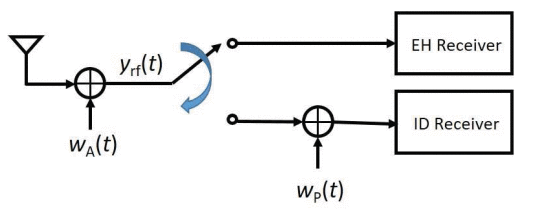
\includegraphics[width=\textwidth]{ts_receiver}
  \caption{Structure of TS receiver \cite{Clerckx2019}}
  \label{fig:ts-receiver}
\end{figure}



\subsection{Power Splitting}\label{sec:power-splitting}
In \textit{Power Splitting} (PS) receiver (Fig. \ref{fig:ps-receiver}), we introduce a PS ratio $\rho $ to split the received signal into individual power stream (with proportion $\rho $) and information stream (with proportion $1 - \rho $). At the transmitter, the signal is jointly optimized for information and power transmission according to CSIT. When perfectly matched, the EH and ID receivers are with input voltage $\sqrt {\rho {R_{{\text{ant}}}}} y(t)$ and $\sqrt {(1 - \rho ){R_{{\text{ant}}}}} y(t)$ respectively. Different rate-energy pairs can be obtained by varying the PS ratio $\rho $. It is argued in \cite{Zhang2013} that PS is the best strategy for linear harvester model with negligible RF-to-baseband noise, but \cite{Clerckx2016} demonstrated that the PS-only transmission is suboptimal when considering rectifier nonlinearity.

\begin{figure}[ht]
  \centering
    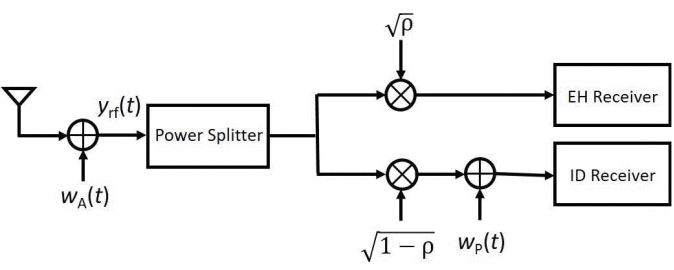
\includegraphics[width=0.8\textwidth]{ps_receiver}
  \caption{Structure of PS receiver \cite{Clerckx2019}}
  \label{fig:ps-receiver}
\end{figure} 